\documentclass[twoside,a4,english,11pt]{book}

\usepackage{hyperref}
\usepackage{fontenc}
\usepackage[latin9]{inputenc}
\usepackage{url}
\usepackage{epsfig}
\usepackage{subfigure}
\usepackage{setspace}
\usepackage{tocbibind}
\usepackage{a4wide}
\usepackage{fullpage}
\usepackage{verbatim}
\usepackage{color,calc}
\usepackage{pdflscape}
\usepackage{fancyvrb}
\usepackage{amsfonts}
\usepackage{listings}

%%%%%%%%%%%%%%%
% DEFINITIONS %
%%%%%%%%%%%%%%%

\urlstyle{leostyle}

\makeatletter
\def\url@leostyle{
  \@ifundefined{selectfont}{\def\UrlFont{\sf}}{\def\UrlFont{\small\ttfamily}}}
\usepackage{babel}
\makeatother

% \setcounter{tocdepth}{0} % Change Table of Contents' depth 

\definecolor{gray}{rgb}{0.4,0.4,0.4}
\definecolor{darkblue}{rgb}{0.0,0.0,0.6}
\definecolor{cyan}{rgb}{0.0,0.6,0.6}
\definecolor{darkgreen}{rgb}{0.33,0.42,0.18}
\definecolor{lightgray}{rgb}{0.8,0.8,0.8}

\def\graybox#1{
  \medskip
  \colorbox{lightgray}{
    \begin{minipage}[t]{0.95\textwidth}
    #1
    \end{minipage}
   }
}

\newcommand{\XTRACK}{{\sf {X}track}\ }

\pagestyle{plain}

%\pagenumbering{roman}

%%%%%%%%%%%%
% DOCUMENT %
%%%%%%%%%%%%

\begin{document}

% \onehalfspacing
% \doublespacing

\title {
  \XTRACK \\
  User Guide
}

\author {
  tools@bsc.es
}

\maketitle
\tableofcontents
% \listoffigures
% \listoftables

\chapter{Xtrack User Guide}

\section{Introduction}

Xtrack is a tool for comparing multiple experiments or different time intervals within the same experiment.
Xtrack takes as input the output produced by the ClusteringSuite tool \cite{BSCTools} as well as the 
output produced by the Extrae On-line module when configured to run automatic structure detection analysis. 
The input of the tool is a series of clustering scatter-plots. Each clustering scatter-plot (or frame) is the 
result of clustering the computations of one execution of a parallel application with respect to selected 
performance metrics. Then, the clusters in one frame represent the main performance trends of the computations 
of the program. Comparing multiple frames, we can study how the behavior of the computing regions change 
between experiments. If we are changing a given parameter between experiments, this is useful to study the 
impact of this parameter in the program performance.

The tool has two parts: the tracking algorithm and the GUI. The \emph{tracking algorithm} takes as 
input the sequence of frames and performs a ``who-is-who'' correlation between the clusters
that appear in all the frames. To do this, the tool applies several heuristics that 
look for different characteristics that can distinguish certain clusters from the others. Then, 
the results of the tracking algorithm can be visualized with the \emph{Xtrack GUI}. 

In this document we briefly introduce the user to both parts of the tool, and show how to use them and 
the different settings available.

\section{The Tracking tool}

The first step to perform this comparative analysis is to apply the tracking algorithm to the sequence of 
frames that results from the application of cluster analyses to different traces (or sub-traces).
To do so, the tool takes as input the list of clustered traces and some optional arguments that define
which heuristics will be used to do the tracking. A detailed description of each of the available 
heuristics can be found here \cite{Llort:IPTW14}. By default, the tool tries to apply all the heuristics
that are applicable with the information comprised in the trace with default settings.

\begin{tabular}{c}
 \tabularnewline
\end{tabular}

\textbf{SYNTAX}
\begin{lstlisting}[frame=single,language=]
  tracking [OPTIONS] [-l LIST | TRACE1 TRACE2 ...]
\end{lstlisting}

\begin{tabular}{c}
 \tabularnewline
\end{tabular}

\textbf{OPTIONS}
\begin{lstlisting}[frame=single,language=]
  -a MIN_SCORE
        Minimum SPMD score to use the alignment tracker
  -c CALLER_LEVEL
        Enable the callers heuristic at the specified stack depth.
  -d MAX_DISTANCE
        Maximum Epsilon distance to use the cross-classifier tracker
  -m MIN_TIME_PCT
        Discard the clusters below the given duration time percentage.
  -s DIM1,DIM2...
        Select the dimensions to scale with the number of tasks.
  -o OUTPUT_PREFIX
        Set the prefix for all the output files.
  -r    Enable the trace reconstruction with tracked clusters.
  -t THRESHOLD
        Minimum likeliness percentage in order to match two clusters 
        (special values: all | first).
  -v[v] Run in verbose mode (-vv for extra debug messages).
  -x CLUSTERING_CONFIG_XML
        Specify the clustering configuration to automatically 
        cluster the traces.
\end{lstlisting}

As a result, the tool generates:

\begin{itemize}
 \item Trajectory lines for all the clusters in the frames, that show how the behavior of the clusters change across experiments.
 \item Recolored frames: a new set of scatter-plots where the identifiers of the clusters and their colors have been changed to make them match across experiments for easy comparison.
 \item Tracked traces: the input trace is reconstructed, changing the clustering events so that the clusters identifiers and their colors are the same in all experiments for easy comparison.
 \item The \emph{*.xtrack} definition file. This file contains all the information about ``who-is-who'' between experiments, and is the input for the Xtrack GUI. 
\end{itemize}

        
\section{The Xtrack GUI}

The Xtrack GUI takes as input the results of applying the tracking algorithm, and displays a graphical comparison of the different experiments. Figure 
\ref{fig:GUI} shows the main view of the tool.

\begin{figure}[t]
\centering
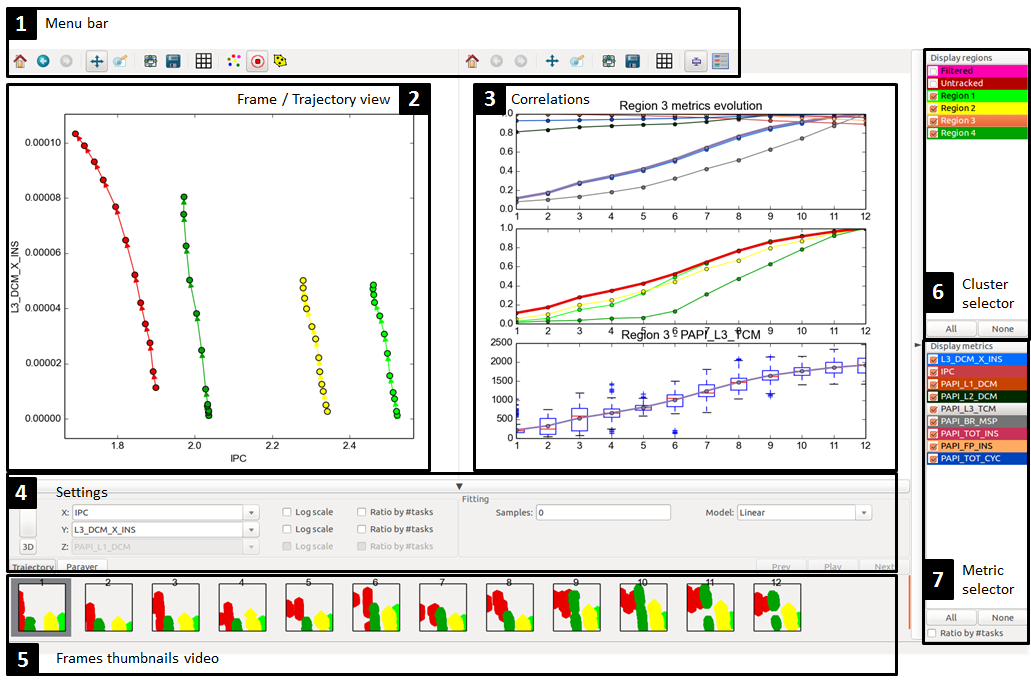
\includegraphics[width=1\textwidth]{imgs/xtrack_gui.png}
\caption{Xtrack GUI}
\label{fig:GUI}
\end{figure}

\subsection{Menu bar}

The menu bar contains controls to manipulate the plotting areas 2 and 3. From left to right, the common controls 
in both bars are:

\begin{itemize}
 \item \textbf{Reset} the plot to the default view.
 \item \textbf{Undo} the last pan or zoom.
 \item \textbf{Redo} the last pan or zoom.
 \item \textbf{Pan} the graph towards any direction.
 \item \textbf{Zoom-in} dragging a box with the left mouse button, or \textbf{zoom-out} with the right mouse button.
 \item Adjust the plot \textbf{margins}.
 \item \textbf{Save} the visible plot.
\end{itemize}

The specific controls for the left menu bar (that controls plotting area 2) are:

\begin{itemize}
 \item Show/hide a \textbf{grid} in the plot.
 \item Show/hide the \textbf{centroids} of the clusters.
 \item Show/hide the \textbf{perimeters} of the clusters.
\end{itemize}

And the specific controls for the right menu bar (that controls plotting area 3) are:

\begin{itemize}
 \item Show/hide \textbf{boxplots} for dispersion plot in pane 3 (dispersion graph).
 \item Show/hide plots \textbf{legends}.
\end{itemize}


\subsection{Frame/Trajectory view}

This is the main view of the tool. When the \emph{frame view} setting is selected in pane 4, it displays the cluster results 
for one single frame of the input sequence of experiments, the one that is selected in pane 5. When the \emph{trajectory view}
is selected in pane 4, it displays instead all the clusters from all the frames at the same time, and draws trajectory lines
that show how the clusters are moving from one experiment to the next. In the image, the trajectory view is set by default.

\subsection{Correlations}

This pane shows correlations for different clusters and metrics across the sequence of experiments (X-axis). The top plot shows a 
correlation of all metrics that are checked in pane 7, for the cluster that is selected in pane 6. The middle plot shows a correlation 
of the selected metric in pane 7, for all the clusters that are checked in pane 6. Since these two plots can display different metrics 
or very different ranges for the same metric in the Y-axis, the value for this axis is normalized. The bottom plot shows the dispersion 
of the selected metric in pane 7 for the selected cluster in pane 6. In this case, the Y-axis shows real values. 

\subsection{Settings}

The settings is divided in two parts. The \emph{Axes} configuration (left) determine the metrics that are used to plot the 
performance space in pane 2. It is possible to select any performance counter that was used to cluster the trace or extrapolated, 
and also to select a third metric to change the view into a 3D plot. The \emph{Log scale} checkbox can be ticked to draw each
axis in logarithmic scale. The \emph{Ratio by \#tasks} can be selected to weight that axis metric with respect to the number 
of tasks that were used in the selected frame. This is useful when the metric is related to the number of instructions executed 
(e.g. total instructions, floating point instructions, etc.) for doing strong scaling or weak scaling comparisons, and studying
code replication issues.

The \emph{Fitting} settings (right) are used to do predictions based on the experiments we have. You can select a fitting model 
between linear, quadratic, cubic, logarithmic or log-linear (right), and a number of experiments to predict (left), and all 
the correlation plots in pane 3 will extend their X-axis to predict how the series will continue according to the selected model.

\subsection{Frame thumbnails video}

This pane shows a carousel of frames, where each frame is the clustering result of every single experiment. This representation 
provides a quick view on the changes across experiments. Also, this pane allows to select a single frame to be inspected in 
detail in pane 2.

\subsection{Cluster selector}

Ticking the checkbox of each cluster we can control whether that cluster has to be displayed/hidden in the plots in panes 2 and 3. Also
selecting a single cluster from the list, changes the plots in pane 3 to display the metrics correlations for the selected cluster only.

\subsection{Metric selector}

Analogously, ticking the checkbox of each metric we can control whether that metric has to be displayed/hidden in the plots in pane 3. 
Also, selecting a single metric from the list, changes the plots in pane 3 to display the correlations of clusters for the selected metric only.

\bibliographystyle{abbrv}
\bibliography{references.bib}

\end{document}